\begin{center}
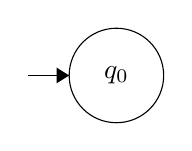
\begin{tikzpicture}[scale=0.2]
\tikzstyle{every node}+=[inner sep=0pt]
\draw [black] (11.8,-27.6) circle (3);
\draw (11.8,-27.6) node {$q_0$};
\draw [black] (6.2,-27.6) -- (8.8,-27.6);
\fill [black] (8.8,-27.6) -- (8,-27.1) -- (8,-28.1);
\end{tikzpicture}
\end{center}